\documentclass[10pt]{beamer}
\usetheme{metropolis}

% ── Packages ──
\usepackage{amsmath,amssymb,amsthm}
\usepackage{tikz}
\usetikzlibrary{positioning,arrows.meta,fit,calc,matrix,shapes.geometric}
\usepackage{graphicx}
\usepackage{array}

% ── Theorem environments ──
\theoremstyle{definition}
\newtheorem{defi}{Definition}[section]
\newtheorem{prop}{Proposition}[section]
\newtheorem{thm}{Theorem}[section]
\newtheorem{cor}{Corollary}[section]

% ── Emoji definitions ──
\newcommand{\bean}{
\includegraphics[scale=0.07]{Pictures/bean.png}}
\newcommand{\leaf}{
\includegraphics[scale=0.08]{Pictures/leaf.png}}
\newcommand{\lemon}{
\includegraphics[scale=0.08]{Pictures/lemon.png}}
\newcommand{\cow}{
\includegraphics[scale=0.08]{Pictures/cow.png}}
\newcommand{\bento}{
\includegraphics[scale=0.08]{Pictures/bento.png}}
\newcommand{\milk}{
\includegraphics[scale=0.08]{Pictures/milk.png}}
\newcommand{\coffee}{
\includegraphics[scale=0.08]{Pictures/coffee.png}}
\newcommand{\tea}{
\includegraphics[scale=0.08]{Pictures/tea.png}}
\newcommand{\soup}{
\includegraphics[scale=0.08]{Pictures/soup.png}}

% ── Highlighting ──
\newcommand{\x}[1]{\alert{\textbf{#1}}}

\title{Lecture 4: Subspace and Linear Independence}
\subtitle{Proving Rank is Well-Defined Through Geometry}
\date{}

\begin{document}
\maketitle

% ═══════════════════════════════════════
% §1 MOTIVATION
% ═══════════════════════════════════════
\section{Motivation: Is Rank Well-Defined?}

\begin{frame}{Recall: Rank from Cross-Filling (Lecture 3)}
In Lecture 3, we defined:

\begin{defi}[Rank — Algorithmic Definition]
$$\text{rank}(A) = \text{number of rank-one pieces from cross-filling}$$
\end{defi}

\vfill
Cross-filling decomposes:
$$A = R_1 + R_2 + \cdots + R_r = UV$$

where each $R_i$ is rank-one, and $r$ is the rank.
\end{frame}

\begin{frame}{The Problem: Different Pivot Choices}
Cross-filling allows \x{different pivot choices} at each step.

\vfill
$$A = \begin{pmatrix} 2 & 4 & 6 \\ 1 & 2 & 3 \\ 3 & 6 & 9 \end{pmatrix}$$

\vfill
We could pick pivot at:
\begin{itemize}
\item Position $(1,1)$ with value 2
\item Position $(2,2)$ with value 2
\item Position $(3,3)$ with value 9
\end{itemize}

\vfill
\x{Question}: Do all choices give the \x{same number} of pieces?
\end{frame}

\begin{frame}{Today's Goal}
\x{Prove that rank is well-defined} by discovering:

$$\boxed{\text{rank}(A) = \text{dimension of column space}}$$

\vfill
\textbf{Strategy}:
\begin{enumerate}
\item Understand \x{two languages} for describing sets
\item Define \x{subspaces} and \x{column space}
\item Introduce \x{linear independence}, \x{basis}, \x{dimension}
\item Prove cross-filling produces a \x{basis} for column space
\item Prove all bases have \x{same size} (using trace)
\item Conclude: rank = dimension (well-defined!)
\end{enumerate}

\vfill
We elevate rank from \x{algorithm} to \x{geometry}.
\end{frame}

% ═══════════════════════════════════════
% §2 TWO LANGUAGES
% ═══════════════════════════════════════
\section{Two Languages for Describing Sets}

\begin{frame}{Daily Life: Finding Your Classroom}
Suppose you want to tell someone \x{where your classroom is}.

\vfill
\textbf{Method A (Descriptive)}: List properties it satisfies
\begin{itemize}
\item "Find the room that has exactly 30 desks"
\item "Has windows facing south"
\item "Is on the 2nd floor"
\end{itemize}

\vfill
\textbf{Method B (Constructive)}: Give directions to generate it
\begin{itemize}
\item "Go to 2nd floor"
\item "Walk to end of hall"
\item "Turn left, last door"
\end{itemize}
\end{frame}

\begin{frame}{Two Languages: Comparison}
\begin{center}
\begin{tabular}{|l|p{3.5cm}|p{3.5cm}|}
\hline
& \textbf{Descriptive} & \textbf{Constructive} \\
\hline
\textbf{How} & List \x{properties} members must satisfy & Provide \x{recipe} to generate members \\
\hline
\textbf{Strength} & Easy to \x{verify} membership & Easy to \x{generate} new members \\
\hline
\textbf{Weakness} & Hard to \x{produce} members & Hard to \x{verify} membership \\
\hline
\textbf{Example} & "Red hat wearers" & "2nd floor, last door left" \\
\hline
\end{tabular}
\end{center}

\vfill
\x{Key}: Neither is better — they're \x{complementary}! We need both.
\end{frame}

\begin{frame}{Example: Line Through Origin in $\mathbb{R}^2$}
Consider the line $y = 2x$:

\vfill
\textbf{Descriptive language} (equation):
$$L = \left\{ \begin{pmatrix} x \\ y \end{pmatrix} : y = 2x \right\}$$

\begin{itemize}
\item To \x{verify} $\begin{pmatrix} 3 \\ 6 \end{pmatrix} \in L$: Check $6 = 2(3)$ $\checkmark$
\item To \x{generate} members: Hard! Need to solve equation
\end{itemize}

\vfill
\textbf{Constructive language} (parametric):
$$L = \left\{ t \begin{pmatrix} 1 \\ 2 \end{pmatrix} : t \in \mathbb{R} \right\}$$

\begin{itemize}
\item To \x{generate} members: Pick any $t$! E.g., $t=3$ gives $\begin{pmatrix} 3 \\ 6 \end{pmatrix}$
\item To \x{verify} $\begin{pmatrix} 3 \\ 6 \end{pmatrix} \in L$: Hard! Find $t$ such that $t\begin{pmatrix} 1 \\ 2 \end{pmatrix} = \begin{pmatrix} 3 \\ 6 \end{pmatrix}$
\end{itemize}
\end{frame}

\begin{frame}{Example: Plane Through Origin in $\mathbb{R}^3$}
\textbf{Descriptive}:
$$P = \left\{ \begin{pmatrix} x \\ y \\ z \end{pmatrix} : x + y + z = 0 \right\}$$

Easy to verify: Check if sum = 0

\vfill
\textbf{Constructive}:
$$P = \left\{ s \begin{pmatrix} 1 \\ 0 \\ -1 \end{pmatrix} + t \begin{pmatrix} 0 \\ 1 \\ -1 \end{pmatrix} : s,t \in \mathbb{R} \right\}$$

Easy to generate: Pick any $s, t$

\vfill
\x{Same plane, two languages!}
\end{frame}

\begin{frame}{Connection to Matrices}
For a matrix $A$:

\vfill
\textbf{Null space} (descriptive):
$$\{ x : Ax = 0 \}$$
Described by an \x{equation} that members must satisfy.

\vfill
\textbf{Column space} (constructive):
$$\{ Ax : x \in \mathbb{R}^n \}$$
Described by a \x{recipe} to generate members.

\end{frame}

\begin{frame}{Solving Equations Overcomes Language Weaknesses}
\x{Constructive language weakness}: Hard to \x{verify} if $b \in \operatorname{Col}(A)$

\vfill
Given $b$, is it a linear combination of columns of $A$? Hard to check directly!

\vfill
\x{How to compensate?} Switch to the \x{descriptive/equation perspective}:

$$\text{Solve } Ax = b$$

\begin{itemize}
\item If solution exists $\to$ $b \in \operatorname{Col}(A)$ $\checkmark$
\item If no solution $\to$ $b \notin \operatorname{Col}(A)$ $\times$
\end{itemize}

\vfill
\x{Key}: \x{Solving equations} is the \x{tool} to overcome constructive language's verification weakness!

Not "understanding language helps solve" — it's "solving helps overcome language limitation".
\end{frame}

% ═══════════════════════════════════════
% §3 SUBSPACES
% ═══════════════════════════════════════
\section{Subspaces: Flat Spaces Through Origin}

\begin{frame}{Definition: Subspace}
\begin{defi}[Subspace]
A \x{subspace} $W$ of $\mathbb{R}^n$ is a non-empty subset that is \x{closed under linear combinations}:

For any $\mathbf{u}, \mathbf{v} \in W$ and any scalars $\alpha, \beta \in \mathbb{R}$:
$$\alpha \mathbf{u} + \beta \mathbf{v} \in W$$
\end{defi}

\vfill
\x{Equivalently}, check these three conditions:
\begin{enumerate}
\item $\mathbf{0} \in W$ (contains zero vector)
\item If $\mathbf{u}, \mathbf{v} \in W$, then $\mathbf{u} + \mathbf{v} \in W$ (closed under addition)
\item If $\mathbf{u} \in W$ and $\alpha \in \mathbb{R}$, then $\alpha \mathbf{u} \in W$ (closed under scaling)
\end{enumerate}
\end{frame}

\begin{frame}{Geometric Intuition: Flat Spaces}
A subspace is a \x{flat space} that:
\begin{itemize}
\item Passes through the \x{origin} (must contain $\mathbf{0}$)
\item Is \x{closed} under vector operations
\end{itemize}

\vfill
\x{Examples of subspaces}:
\begin{itemize}
\item Lines through origin in $\mathbb{R}^2$ or $\mathbb{R}^3$
\item Planes through origin in $\mathbb{R}^3$
\item All of $\mathbb{R}^n$ itself
\item Just $\{\mathbf{0}\}$ (the zero subspace)
\end{itemize}

\vfill
\x{Non-examples}:
\begin{itemize}
\item Line $y = 2x + 1$ (doesn't pass through origin)
\item Unit circle (not closed under scaling: $2 \cdot \begin{pmatrix} 1 \\ 0 \end{pmatrix}$ not on circle)
\end{itemize}
\end{frame}

\begin{frame}{Example: Verifying a Subspace}
\textbf{Question}: Is $W = \left\{ \begin{pmatrix} x \\ y \\ z \end{pmatrix} : x + 2y - z = 0 \right\}$ a subspace of $\mathbb{R}^3$?

\vfill
\textbf{Step 1}: Check $\mathbf{0} \in W$

$$\begin{pmatrix} 0 \\ 0 \\ 0 \end{pmatrix}: \quad 0 + 2(0) - 0 = 0 \quad \checkmark$$

\vfill
\textbf{Step 2}: Check closure under linear combinations

Take any $\mathbf{u}, \mathbf{v} \in W$. Then:
\begin{itemize}
\item $u_1 + 2u_2 - u_3 = 0$ (since $\mathbf{u} \in W$)
\item $v_1 + 2v_2 - v_3 = 0$ (since $\mathbf{v} \in W$)
\end{itemize}
\end{frame}

\begin{frame}{Example: Verifying a Subspace (continued)}
For any scalars $\alpha, \beta$, check $\alpha\mathbf{u} + \beta\mathbf{v} \in W$:

$$\alpha\mathbf{u} + \beta\mathbf{v} = \begin{pmatrix} \alpha u_1 + \beta v_1 \\ \alpha u_2 + \beta v_2 \\ \alpha u_3 + \beta v_3 \end{pmatrix}$$

\vfill
Verify the equation:
\begin{align*}
&(\alpha u_1 + \beta v_1) + 2(\alpha u_2 + \beta v_2) - (\alpha u_3 + \beta v_3) \\
&= \alpha(u_1 + 2u_2 - u_3) + \beta(v_1 + 2v_2 - v_3) \\
&= \alpha(0) + \beta(0) = 0 \quad \checkmark
\end{align*}

\vfill
\x{Conclusion}: $W$ is a subspace! (It's a plane through origin)
\end{frame}

\begin{frame}{Non-Example: Line Not Through Origin}
\textbf{Question}: Is $U = \left\{ \begin{pmatrix} x \\ y \end{pmatrix} : x + y = 1 \right\}$ a subspace?

\vfill
\x{Quick check}: Is $\mathbf{0} \in U$?

$$\begin{pmatrix} 0 \\ 0 \end{pmatrix}: \quad 0 + 0 = 0 \neq 1 \quad \times$$

\vfill
\x{Conclusion}: NOT a subspace!

This is a line not through the origin.
\end{frame}

% ═══════════════════════════════════════
% §4 COLUMN SPACE
% ═══════════════════════════════════════
\section{Column Space: The Constructive Subspace}

\begin{frame}{Definition: Column Space}
\begin{defi}[Column Space]
For an $m \times n$ matrix $A = \begin{pmatrix} | & & | \\ \mathbf{a}_1 & \cdots & \mathbf{a}_n \\ | & & | \end{pmatrix}$:

$$\operatorname{Col}(A) = \{ Ax : x \in \mathbb{R}^n \}$$

\textbf{Equivalently} (column combination view):
$$\operatorname{Col}(A) = \{ x_1 \mathbf{a}_1 + \cdots + x_n \mathbf{a}_n : x_1, \ldots, x_n \in \mathbb{R} \}$$

This is the set of \x{all linear combinations of columns} of $A$.
\end{defi}

\vfill
\x{Language}: Column space is \x{constructive} — defined by a \x{recipe}!

Pick coefficients $x_1, \ldots, x_n$, form the combination.
\end{frame}

\begin{frame}{Column Space is a Subspace}
\begin{prop}
$\operatorname{Col}(A)$ is a subspace of $\mathbb{R}^m$.
\end{prop}

\vfill
\textbf{Proof}:

\textbf{(1)} Contains $\mathbf{0}$: Take $x = \mathbf{0}$, then $A\mathbf{0} = \mathbf{0} \in \operatorname{Col}(A)$ $\checkmark$

\vfill
\textbf{(2)} Closed under linear combinations:
\begin{itemize}
\item Take $\mathbf{b}_1, \mathbf{b}_2 \in \operatorname{Col}(A)$
\item Then $\mathbf{b}_1 = Ax_1$ and $\mathbf{b}_2 = Ax_2$ for some $x_1, x_2$
\item For any $\alpha, \beta$:
$$\alpha\mathbf{b}_1 + \beta\mathbf{b}_2 = \alpha Ax_1 + \beta Ax_2 = A(\alpha x_1 + \beta x_2) \in \operatorname{Col}(A)$$
\end{itemize}

$\checkmark$ Therefore $\operatorname{Col}(A)$ is a subspace!
\end{frame}

\begin{frame}{Example: Column Space of Rank-One Matrix}
$$A = \begin{pmatrix} 2 & 4 & 6 \\ 1 & 2 & 3 \end{pmatrix} = \begin{pmatrix} 2 \\ 1 \end{pmatrix} \begin{pmatrix} 1 & 2 & 3 \end{pmatrix}$$

\vfill
All columns are multiples of $\begin{pmatrix} 2 \\ 1 \end{pmatrix}$:

$$\operatorname{Col}(A) = \left\{ t \begin{pmatrix} 2 \\ 1 \end{pmatrix} : t \in \mathbb{R} \right\}$$

\vfill
This is a \x{line through origin} in $\mathbb{R}^2$!

\vfill
Visual: All points on line $y = \frac{1}{2}x$.
\end{frame}

\begin{frame}{Connection to Solvability (Lecture 3 Recall)}
Recall from Lecture 3:

$$Ax = b \text{ has a solution} \quad \Longleftrightarrow \quad b \in \operatorname{Col}(A)$$

\vfill
\x{Why?}

Because $Ax$ is a linear combination of columns of $A$, and $\operatorname{Col}(A)$ is \x{exactly} the set of all such combinations!

\vfill
\x{Column space captures which vectors can be produced} by $A$.
\end{frame}

% ═══════════════════════════════════════
% §5 LINEAR INDEPENDENCE
% ═══════════════════════════════════════
\section{Linear Independence and Span}

\begin{frame}{Motivation: Redundant Recipe Vectors}
Shinchan's coffee shop has recipe vectors (columns = ingredients):

\begin{center}
\begin{tabular}{c|ccc}
& \coffee & \tea & \soup \\
\hline
\bean & 2 & 1 & 3 \\
\leaf & 1 & 2 & 3 \\
\lemon & 0 & 1 & 1
\end{tabular}
\end{center}

\vfill
\x{Question}: Is \soup~redundant?

Notice: \soup~= \coffee~+ \tea~(ingredient-wise)

$$\begin{pmatrix} 3 \\ 3 \\ 1 \end{pmatrix} = \begin{pmatrix} 2 \\ 1 \\ 0 \end{pmatrix} + \begin{pmatrix} 1 \\ 2 \\ 1 \end{pmatrix}$$

\vfill
\x{Yes!} We can remove \soup~and still make everything.

This is \x{linear dependence}.
\end{frame}

\begin{frame}{The Real Question: Minimum Generators}
\x{Motivation for Linear Independence}:

\vfill
\textbf{Problem}: Given recipe vectors $v_1, v_2, \ldots, v_k$:
\begin{itemize}
\item Can we write one using the others? (redundancy)
\item Can we \x{remove} some and still generate everything?
\item What's the \x{minimum set} needed?
\end{itemize}

\vfill
\textbf{Goal}: Find vectors with \x{no redundancy} — each contributes something \x{new}.

\vfill
This concept is called \x{linear independence}.
\end{frame}

\begin{frame}{Definition: Linear Independence}
\begin{defi}[Linearly Independent]
Vectors $\mathbf{v}_1, \ldots, \mathbf{v}_k$ are \x{linearly independent} if:

$$c_1\mathbf{v}_1 + \cdots + c_k\mathbf{v}_k = \mathbf{0} \quad \Rightarrow \quad c_1 = \cdots = c_k = 0$$
\end{defi}

\vfill
\x{Intuition}: The only way to combine them to get zero is the trivial way (all coefficients zero).

\vfill
\x{Contrapositive interpretation}: No vector can be written as a combination of the others.

\vfill
\begin{defi}[Linearly Dependent]
If there exists a \x{non-trivial} combination giving zero:
$$c_1\mathbf{v}_1 + \cdots + c_k\mathbf{v}_k = \mathbf{0} \quad \text{with some } c_i \neq 0$$
\end{defi}
\end{frame}

\begin{frame}{Why This Definition Captures Redundancy}
If \x{dependent}, say $c_1\mathbf{v}_1 + \cdots + c_k\mathbf{v}_k = \mathbf{0}$ with $c_1 \neq 0$:

$$c_1\mathbf{v}_1 = -c_2\mathbf{v}_2 - \cdots - c_k\mathbf{v}_k$$

$$\mathbf{v}_1 = -\frac{c_2}{c_1}\mathbf{v}_2 - \cdots - \frac{c_k}{c_1}\mathbf{v}_k$$

\vfill
$\mathbf{v}_1$ can be written using the others — \x{redundant}!

\vfill
If \x{independent}, no such representation exists — \x{no redundancy}.
\end{frame}

\begin{frame}{Example: Testing Independence}
Are $\begin{pmatrix} 1 \\ 0 \end{pmatrix}, \begin{pmatrix} 0 \\ 1 \end{pmatrix}$ linearly independent?

\vfill
\textbf{Test}: Check $c_1\begin{pmatrix} 1 \\ 0 \end{pmatrix} + c_2\begin{pmatrix} 0 \\ 1 \end{pmatrix} = \begin{pmatrix} 0 \\ 0 \end{pmatrix}$

$$\begin{pmatrix} c_1 \\ c_2 \end{pmatrix} = \begin{pmatrix} 0 \\ 0 \end{pmatrix}$$

\vfill
Only solution: $c_1 = 0, c_2 = 0$ $\checkmark$

\vfill
\x{Conclusion}: Linearly independent!
\end{frame}

\begin{frame}{Example: Detecting Dependence}
Are $\begin{pmatrix} 2 \\ 1 \end{pmatrix}, \begin{pmatrix} 4 \\ 2 \end{pmatrix}, \begin{pmatrix} 6 \\ 3 \end{pmatrix}$ linearly independent?

\vfill
\textbf{Observe}: Column 2 = 2$\cdot$Column 1, Column 3 = 3$\cdot$Column 1

\vfill
Try $c_1 = 3, c_2 = 0, c_3 = -1$:
$$3\begin{pmatrix} 2 \\ 1 \end{pmatrix} + 0\begin{pmatrix} 4 \\ 2 \end{pmatrix} - 1\begin{pmatrix} 6 \\ 3 \end{pmatrix} = \begin{pmatrix} 6 \\ 3 \end{pmatrix} - \begin{pmatrix} 6 \\ 3 \end{pmatrix} = \begin{pmatrix} 0 \\ 0 \end{pmatrix}$$

\vfill
\x{Non-trivial solution exists!}

\vfill
\x{Conclusion}: Linearly \x{dependent}!
\end{frame}

\begin{frame}{Definition: Span}
\begin{defi}[Span]
The \x{span} of vectors $\mathbf{v}_1, \ldots, \mathbf{v}_k$ is the set of all their linear combinations:

$$\operatorname{span}\{\mathbf{v}_1, \ldots, \mathbf{v}_k\} = \{ c_1\mathbf{v}_1 + \cdots + c_k\mathbf{v}_k : c_1, \ldots, c_k \in \mathbb{R} \}$$

We say $\{\mathbf{v}_1, \ldots, \mathbf{v}_k\}$ \x{spans} $W$ if $\operatorname{span}\{\mathbf{v}_1, \ldots, \mathbf{v}_k\} = W$.
\end{defi}

\vfill
\x{Connection to column space}:
$$\operatorname{Col}(A) = \operatorname{span}\{\text{columns of } A\}$$

They're the same thing!
\end{frame}

% ═══════════════════════════════════════
% §6 BASIS
% ═══════════════════════════════════════
\section{Basis: Minimal Spanning Sets}

\begin{frame}{Definition: Basis}
\begin{defi}[Basis]
A \x{basis} for a subspace $W$ is a list of vectors that:
\begin{enumerate}
\item \x{Spans} $W$ (every vector in $W$ can be written as their combination)
\item Is \x{linearly independent} (no redundancy)
\end{enumerate}

\textbf{Equivalently}: A basis is a \x{minimal spanning set} or a \x{maximal independent set}.
\end{defi}

\vfill
\x{Key property}: A basis gives \x{unique coordinates}!

If $\{\mathbf{e}_1, \ldots, \mathbf{e}_r\}$ is a basis, then \x{every} $\mathbf{v} \in W$ can be written \x{uniquely} as:
$$\mathbf{v} = c_1\mathbf{e}_1 + \cdots + c_r\mathbf{e}_r$$
\end{frame}

\begin{frame}{Why Basis Gives Unique Coordinates}
\textbf{Existence}: Spanning ensures you can write $\mathbf{v}$ as a combination.

\vfill
\textbf{Uniqueness}: Suppose two representations:
$$\mathbf{v} = c_1\mathbf{e}_1 + \cdots + c_r\mathbf{e}_r = d_1\mathbf{e}_1 + \cdots + d_r\mathbf{e}_r$$

Then:
$$(c_1 - d_1)\mathbf{e}_1 + \cdots + (c_r - d_r)\mathbf{e}_r = \mathbf{0}$$

By linear independence, all $c_i - d_i = 0$, so $c_i = d_i$ for all $i$. $\checkmark$

\vfill
\x{Basis = efficient coordinate system with no redundancy!}
\end{frame}

\begin{frame}{Example: Standard Basis for $\mathbb{R}^3$}
$$\mathbf{e}_1 = \begin{pmatrix} 1 \\ 0 \\ 0 \end{pmatrix}, \quad \mathbf{e}_2 = \begin{pmatrix} 0 \\ 1 \\ 0 \end{pmatrix}, \quad \mathbf{e}_3 = \begin{pmatrix} 0 \\ 0 \\ 1 \end{pmatrix}$$

\vfill
\textbf{Check independence}:
$$c_1\mathbf{e}_1 + c_2\mathbf{e}_2 + c_3\mathbf{e}_3 = \begin{pmatrix} c_1 \\ c_2 \\ c_3 \end{pmatrix} = \mathbf{0}$$
Only if all $c_i = 0$ $\checkmark$

\vfill
\textbf{Check spanning}:
Any $\begin{pmatrix} x \\ y \\ z \end{pmatrix} = x\mathbf{e}_1 + y\mathbf{e}_2 + z\mathbf{e}_3$ $\checkmark$

\vfill
\x{Conclusion}: $\{\mathbf{e}_1, \mathbf{e}_2, \mathbf{e}_3\}$ is a basis for $\mathbb{R}^3$!
\end{frame}

\begin{frame}{Example: Another Basis for $\mathbb{R}^2$}
$$\mathbf{v}_1 = \begin{pmatrix} 1 \\ 1 \end{pmatrix}, \quad \mathbf{v}_2 = \begin{pmatrix} 1 \\ -1 \end{pmatrix}$$

\vfill
\textbf{Check independence}: From $c_1\mathbf{v}_1 + c_2\mathbf{v}_2 = \mathbf{0}$:
$$c_1 + c_2 = 0, \quad c_1 - c_2 = 0$$
Add: $2c_1 = 0 \Rightarrow c_1 = 0 \Rightarrow c_2 = 0$ $\checkmark$

\vfill
\textbf{Check spanning}: For any $\begin{pmatrix} x \\ y \end{pmatrix}$, solve:
$$c_1 + c_2 = x, \quad c_1 - c_2 = y$$

Solution: $c_1 = \frac{x+y}{2}, c_2 = \frac{x-y}{2}$ (always exists!) $\checkmark$

\vfill
\x{Conclusion}: $\{\mathbf{v}_1, \mathbf{v}_2\}$ is another basis for $\mathbb{R}^2$!
\end{frame}

% ═══════════════════════════════════════
% §7 LEFT CANCELLATION
% ═══════════════════════════════════════
\section{Left Cancellation Property}

\begin{frame}{Matrix Form of Independence}
Collect vectors $v_1, \ldots, v_k$ as columns of matrix $U$:

$$U = \begin{pmatrix} | & | & & | \\ v_1 & v_2 & \cdots & v_k \\ | & | & & | \end{pmatrix}$$

\vfill
\x{Linear independence} says:
$$U\begin{pmatrix} c_1 \\ \vdots \\ c_k \end{pmatrix} = \mathbf{0} \quad \Rightarrow \quad \begin{pmatrix} c_1 \\ \vdots \\ c_k \end{pmatrix} = \mathbf{0}$$

In other words: $Uc = \mathbf{0} \Rightarrow c = \mathbf{0}$
\end{frame}

\begin{frame}{Left Cancellation Property — Setup}
\begin{prop}[Left Cancellation]
If $U$ has linearly independent columns, then:
$$UP = UQ \quad \Rightarrow \quad P = Q$$
\end{prop}

\vfill
Let's write out what each matrix looks like:

$$U = \begin{pmatrix} | & | & & | \\ \mathbf{u}_1 & \mathbf{u}_2 & \cdots & \mathbf{u}_k \\ | & | & & | \end{pmatrix}$$

$$P = \begin{pmatrix} | & | & & | \\ \mathbf{p}_1 & \mathbf{p}_2 & \cdots & \mathbf{p}_m \\ | & | & & | \end{pmatrix}, \quad Q = \begin{pmatrix} | & | & & | \\ \mathbf{q}_1 & \mathbf{q}_2 & \cdots & \mathbf{q}_m \\ | & | & & | \end{pmatrix}$$

\vfill
$U$ is $n \times k$, $P$ and $Q$ are $k \times m$.
\end{frame}

\begin{frame}{Left Cancellation — What Does $UP$ Mean?}
$$UP = \begin{pmatrix} | & | & & | \\ \mathbf{u}_1 & \mathbf{u}_2 & \cdots & \mathbf{u}_k \\ | & | & & | \end{pmatrix}\begin{pmatrix} | & | & & | \\ \mathbf{p}_1 & \mathbf{p}_2 & \cdots & \mathbf{p}_m \\ | & | & & | \end{pmatrix}$$

\vfill
\x{Column $j$ of $UP$} is:
$$U\mathbf{p}_j = p_{1j}\mathbf{u}_1 + p_{2j}\mathbf{u}_2 + \cdots + p_{kj}\mathbf{u}_k$$

\vfill
This is a \x{linear combination of $U$'s columns} with coefficients from $\mathbf{p}_j$!

\vfill
So:
$$UP = \begin{pmatrix} | & | & & | \\ U\mathbf{p}_1 & U\mathbf{p}_2 & \cdots & U\mathbf{p}_m \\ | & | & & | \end{pmatrix}$$
\end{frame}

\begin{frame}{Left Cancellation — Column-by-Column}
Similarly:
$$UQ = \begin{pmatrix} | & | & & | \\ U\mathbf{q}_1 & U\mathbf{q}_2 & \cdots & U\mathbf{q}_m \\ | & | & & | \end{pmatrix}$$

\vfill
If $UP = UQ$, then \x{column-by-column}:
$$U\mathbf{p}_j = U\mathbf{q}_j \quad \text{for each } j = 1, 2, \ldots, m$$

\vfill
Rearranging:
$$U\mathbf{p}_j - U\mathbf{q}_j = \mathbf{0}$$
$$U(\mathbf{p}_j - \mathbf{q}_j) = \mathbf{0}$$
\end{frame}

\begin{frame}{Left Cancellation — Using Independence}
For each column $j$, we have:
$$U(\mathbf{p}_j - \mathbf{q}_j) = \mathbf{0}$$

\vfill
Expanding:
$$(\mathbf{p}_j - \mathbf{q}_j) = \begin{pmatrix} p_{1j} - q_{1j} \\ p_{2j} - q_{2j} \\ \vdots \\ p_{kj} - q_{kj} \end{pmatrix}$$

$$U(\mathbf{p}_j - \mathbf{q}_j) = (p_{1j} - q_{1j})\mathbf{u}_1 + (p_{2j} - q_{2j})\mathbf{u}_2 + \cdots + (p_{kj} - q_{kj})\mathbf{u}_k = \mathbf{0}$$

\vfill
Since $\{\mathbf{u}_1, \ldots, \mathbf{u}_k\}$ are \x{linearly independent}:
$$p_{1j} - q_{1j} = 0, \quad p_{2j} - q_{2j} = 0, \quad \ldots, \quad p_{kj} - q_{kj} = 0$$
\end{frame}

\begin{frame}{Left Cancellation — Conclusion}
Therefore, for each $j$:
$$\mathbf{p}_j = \mathbf{q}_j$$

\vfill
Since this holds for \x{all columns} $j = 1, 2, \ldots, m$:

$$P = \begin{pmatrix} | & | & & | \\ \mathbf{p}_1 & \mathbf{p}_2 & \cdots & \mathbf{p}_m \\ | & | & & | \end{pmatrix} = \begin{pmatrix} | & | & & | \\ \mathbf{q}_1 & \mathbf{q}_2 & \cdots & \mathbf{q}_m \\ | & | & & | \end{pmatrix} = Q$$

\vfill
$$\boxed{P = Q}$$ $\square$

\vfill
\x{Key step}: Independence of $U$'s columns forces each coefficient difference to be zero.
\end{frame}

\begin{frame}{Why "Left" Cancellation?}
The matrix $U$ appears on the \x{left} in $UP = UQ$, and we can "cancel" it.

\vfill
\x{Contrast}: If columns are \x{dependent}, we \x{cannot} cancel!

\vfill
\textbf{Example}:
$$\begin{pmatrix} 1 & 2 \\ 1 & 2 \end{pmatrix}\begin{pmatrix} 1 \\ 0 \end{pmatrix} = \begin{pmatrix} 1 & 2 \\ 1 & 2 \end{pmatrix}\begin{pmatrix} 0 \\ 0.5 \end{pmatrix} = \begin{pmatrix} 1 \\ 1 \end{pmatrix}$$

But $\begin{pmatrix} 1 \\ 0 \end{pmatrix} \neq \begin{pmatrix} 0 \\ 0.5 \end{pmatrix}$!

Cancellation \x{fails} because columns are dependent.
\end{frame}

\begin{frame}{Consequence: Unique Representation}
If $\{v_1, \ldots, v_k\}$ are linearly independent and:
$$w = c_1v_1 + \cdots + c_kv_k$$

then the coefficients $c_1, \ldots, c_k$ are \x{unique}.

\vfill
\textbf{Proof}: If also $w = d_1v_1 + \cdots + d_kv_k$, then in matrix form:

$$U\begin{pmatrix} c_1 \\ \vdots \\ c_k \end{pmatrix} = U\begin{pmatrix} d_1 \\ \vdots \\ d_k \end{pmatrix}$$

By left cancellation: $c_i = d_i$ for all $i$. $\square$
\end{frame}

% ═══════════════════════════════════════
% §8 CROSS-FILLING PRODUCES BASIS
% ═══════════════════════════════════════
\section{Cross-Filling Produces a Basis}

\begin{frame}{Recall: Cross-Filling (Lecture 3)}
Cross-filling decomposes:
$$A = R_1 + R_2 + \cdots + R_r = UV$$

where:
\begin{itemize}
\item Each $R_i = \mathbf{u}_i\mathbf{v}_i^T$ is rank-one
\item $U = \begin{pmatrix} | & & | \\ \mathbf{u}_1 & \cdots & \mathbf{u}_r \\ | & & | \end{pmatrix}$ collects the column vectors
\item $V = \begin{pmatrix} - & \mathbf{v}_1^T & - \\ & \vdots & \\ - & \mathbf{v}_r^T & - \end{pmatrix}$ collects the row vectors
\end{itemize}

\vfill
\x{Key question}: What is special about $U$'s columns?
\end{frame}

\begin{frame}{Property 1: $U$'s Columns Are Independent}
\begin{prop}
Let $A = UV$ from cross-filling. Then the columns of $U$ are \x{linearly independent}.
\end{prop}

\vfill
\textbf{Proof idea}: Use the \x{pivot structure}!

Each $\mathbf{u}_i$ came from a rank-one piece with pivot in some row $p_i$.

After peeling $R_1, \ldots, R_{i-1}$, rows $p_1, \ldots, p_{i-1}$ of the remainder are \x{zero}.

This creates a \x{triangular pattern} that forces independence.
\end{frame}

\begin{frame}[fragile]{Concrete Example: Step-by-Step Cross-Filling}
Let's do cross-filling on:
$$A = \begin{pmatrix} 2 & 4 & 6 \\ 1 & 2 & 4 \\ 3 & 6 & 9 \end{pmatrix}$$

\vfill
\textbf{Step 1}: Pick pivot at position (row 1, column 1), value 2

\begin{center}
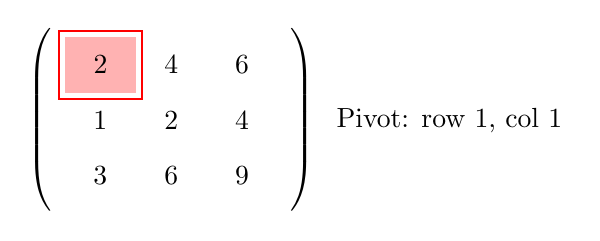
\begin{tikzpicture}[scale=0.9]
\matrix (m) [matrix of math nodes, left delimiter=(, right delimiter=), nodes={minimum width=0.9cm, minimum height=0.7cm}] {
  |[fill=red!30]| 2 & 4 & 6 \\
  1 & 2 & 4 \\
  3 & 6 & 9 \\
};
\node[draw=red, thick, fit=(m-1-1), inner sep=2pt] {};
\node[right=0.5cm of m] {Pivot: row 1, col 1};
\end{tikzpicture}
\end{center}

\vfill
Extract:
$$R_1 = \underbrace{\begin{pmatrix} 2 \\ 1 \\ 3 \end{pmatrix}}_{\mathbf{u}_1 = \text{column 1}} \cdot \underbrace{\begin{pmatrix} 1 & 2 & 3 \end{pmatrix}}_{\mathbf{v}_1^T = \text{row 1}/2}$$
\end{frame}

\begin{frame}[fragile]{Step 2: After Peeling $R_1$}
Remainder:
$$A_2 = A - R_1 = \begin{pmatrix} 2 & 4 & 6 \\ 1 & 2 & 4 \\ 3 & 6 & 9 \end{pmatrix} - \begin{pmatrix} 2 & 4 & 6 \\ 1 & 2 & 3 \\ 3 & 6 & 9 \end{pmatrix} = \begin{pmatrix} 0 & 0 & 0 \\ 0 & 0 & 1 \\ 0 & 0 & 0 \end{pmatrix}$$

\vfill
\begin{center}
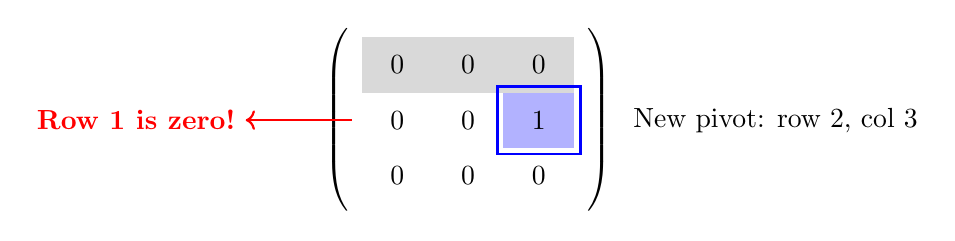
\begin{tikzpicture}[scale=0.9]
\matrix (m) [matrix of math nodes, left delimiter=(, right delimiter=), nodes={minimum width=0.9cm, minimum height=0.7cm}] {
  |[fill=gray!30]| 0 & |[fill=gray!30]| 0 & |[fill=gray!30]| 0 \\
  0 & 0 & |[fill=blue!30]| 1 \\
  0 & 0 & 0 \\
};
\node[draw=blue, thick, fit=(m-2-3), inner sep=2pt] {};
\node[right=0.5cm of m] {New pivot: row 2, col 3};
\draw[->,red,thick] (m.west) -- ++(-1.5,0) node[left] {\textbf{Row 1 is zero!}};
\end{tikzpicture}
\end{center}

\vfill
\x{Key}: After peeling $R_1$, \x{row 1 (the pivot row) became zero}!
\end{frame}

\begin{frame}[fragile]{Step 3: Extract $R_2$}
From remainder $A_2 = \begin{pmatrix} 0 & 0 & 0 \\ 0 & 0 & 1 \\ 0 & 0 & 0 \end{pmatrix}$, pivot at (row 2, col 3):

\vfill
Extract:
$$R_2 = \underbrace{\begin{pmatrix} 0 \\ 1 \\ 0 \end{pmatrix}}_{\mathbf{u}_2 = \text{column 3}} \cdot \underbrace{\begin{pmatrix} 0 & 0 & 1 \end{pmatrix}}_{\mathbf{v}_2^T = \text{row 2}}$$

\vfill
\x{Observe $\mathbf{u}_2$}:
$$\mathbf{u}_2 = \begin{pmatrix} \textcolor{red}{0} \\ 1 \\ 0 \end{pmatrix} \quad \leftarrow \text{First entry is \textcolor{red}{0}}!$$

\vfill
Why? Because row 1 of $A_2$ was already zero, so column 3 of $A_2$ has 0 in row 1.
\end{frame}

\begin{frame}[fragile]{The Pivot Pattern Creates Triangular Structure}
Collected columns:
$$U = \begin{pmatrix} \mathbf{u}_1 & \mathbf{u}_2 \end{pmatrix} = \begin{pmatrix} 2 & \textcolor{red}{0} \\ 1 & 1 \\ 3 & 0 \end{pmatrix}$$

\vfill
\begin{center}
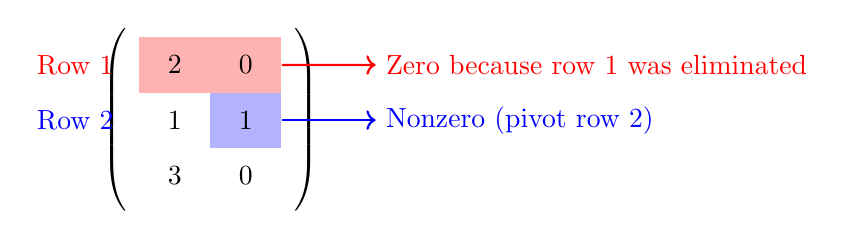
\begin{tikzpicture}[scale=1.1]
\matrix (m) [matrix of math nodes, left delimiter=(, right delimiter=), nodes={minimum width=0.9cm, minimum height=0.7cm}] {
  |[fill=red!30]| 2 & |[fill=red!30]| 0 \\
  1 & |[fill=blue!30]| 1 \\
  3 & 0 \\
};
\draw[->,red,thick] (m-1-2) -- ++(1.5,0) node[right] {Zero because row 1 was eliminated};
\draw[->,blue,thick] (m-2-2) -- ++(1.5,0) node[right] {Nonzero (pivot row 2)};
\node[left=0.2cm of m-1-1] {\textcolor{red}{Row 1}};
\node[left=0.2cm of m-2-1] {\textcolor{blue}{Row 2}};
\end{tikzpicture}
\end{center}

\vfill
\x{Pattern}: $\mathbf{u}_2$ has \x{zero in all previous pivot rows} (row 1).

This is the \x{triangular structure}!
\end{frame}

\begin{frame}{Visual Summary: Why Independence?}
$$U = \begin{pmatrix}
\tikz[baseline=(char.base)]{\node[fill=red!30] (char) {2};} & \tikz[baseline=(char.base)]{\node[fill=red!30] (char) {0};} \\
1 & \tikz[baseline=(char.base)]{\node[fill=blue!30] (char) {1};} \\
3 & 0
\end{pmatrix}$$

\vfill
Check $c_1\mathbf{u}_1 + c_2\mathbf{u}_2 = \mathbf{0}$:

\begin{itemize}
\item \x{Row 1}: $\tikz[baseline=(char.base)]{\node[fill=red!30] (char) {$2c_1$};} + \tikz[baseline=(char.base)]{\node[fill=red!30] (char) {$0 \cdot c_2$};} = 0 \Rightarrow c_1 = 0$
\item \x{Row 2}: $1c_1 + \tikz[baseline=(char.base)]{\node[fill=blue!30] (char) {$1 \cdot c_2$};} = 0 + c_2 = 0 \Rightarrow c_2 = 0$
\end{itemize}

\vfill
The triangular pattern (zeros in previous pivot rows) allows \x{backward substitution}!

\vfill
We can solve from top to bottom, determining each $c_i = 0$ uniquely.
\end{frame}

\begin{frame}{Checking Independence by Backward Substitution}
Check: $c_1\mathbf{u}_1 + c_2\mathbf{u}_2 = \mathbf{0}$

$$c_1\begin{pmatrix} 2 \\ 1 \\ 3 \end{pmatrix} + c_2\begin{pmatrix} 0 \\ 1 \\ 0 \end{pmatrix} = \begin{pmatrix} 2c_1 \\ c_1 + c_2 \\ 3c_1 \end{pmatrix} = \begin{pmatrix} 0 \\ 0 \\ 0 \end{pmatrix}$$

\vfill
\textbf{Solve backwards} (using triangular structure):
\begin{itemize}
\item Row 3: $3c_1 = 0 \Rightarrow c_1 = 0$
\item Row 1: $2c_1 = 0$ $\checkmark$ (consistent)
\item Row 2: $c_1 + c_2 = 0 + c_2 = 0 \Rightarrow c_2 = 0$
\end{itemize}

\vfill
All coefficients zero! Independent $\checkmark$
\end{frame}

\begin{frame}{General Proof: Pivot Row Method}
Let $\mathbf{u}_1, \ldots, \mathbf{u}_r$ be columns from cross-filling, where $\mathbf{u}_i$ has pivot in row $p_i$.

\vfill
\x{Key observation}: After peeling $R_1, \ldots, R_{i-1}$, rows $p_1, \ldots, p_{i-1}$ of remainder are zero.

Therefore:
$$\mathbf{u}_i[\text{row } p_j] = 0 \quad \text{for all } j < i$$

\vfill
\textbf{Check independence}: Suppose $c_1\mathbf{u}_1 + \cdots + c_r\mathbf{u}_r = \mathbf{0}$.

\x{Solve backwards}:
\begin{enumerate}
\item Look at pivot row $p_r$: Only $\mathbf{u}_r$ has nonzero entry there, so $c_r = 0$
\item Look at pivot row $p_{r-1}$: Only $\mathbf{u}_{r-1}$ and $\mathbf{u}_r$ could contribute, but $c_r = 0$, so $c_{r-1} = 0$
\item Continue: $c_{r-2} = 0, \ldots, c_1 = 0$
\end{enumerate}

All coefficients zero! $\checkmark$
\end{frame}

\begin{frame}{Property 2: $\operatorname{Col}(U) = \operatorname{Col}(A)$}
\begin{prop}
If $A = UV$ from cross-filling, then:
$$\operatorname{Col}(U) = \operatorname{Col}(A)$$
\end{prop}

\vfill
\textbf{Proof (Two inclusions)}:

\x{Part 1}: $\operatorname{Col}(A) \subseteq \operatorname{Col}(U)$

Since $A = UV$:
$$Ax = UV x = U(Vx)$$

Let $y = Vx$, then $Ax = Uy \in \operatorname{Col}(U)$ $\checkmark$
\end{frame}

\begin{frame}{Property 2 (continued): The Deeper Direction}
\x{Part 2}: $\operatorname{Col}(U) \subseteq \operatorname{Col}(A)$

Must show: Every column of $U$ is in $\operatorname{Col}(A)$.

\vfill
\textbf{Key idea}: Cross-filling \x{peels columns from $A$}!

Each $\mathbf{u}_i$ comes from a column of some remainder matrix $A_k$.

Remainders are built from $A$'s columns, so $\mathbf{u}_i \in \operatorname{Col}(A)$.
\end{frame}

\begin{frame}{Detailed Argument: Induction on Remainders}
Cross-filling process:
\begin{itemize}
\item Start: $A_1 = A$
\item Peel $R_1 = \mathbf{u}_1\mathbf{v}_1^T$ where $\mathbf{u}_1$ is (scaled) column of $A_1$
\item Remainder: $A_2 = A_1 - R_1$
\item Peel $R_2 = \mathbf{u}_2\mathbf{v}_2^T$ where $\mathbf{u}_2$ is (scaled) column of $A_2$
\item Continue...
\end{itemize}

\vfill
\x{Claim}: Every column of $A_k$ is in $\operatorname{Col}(A)$.

\textbf{Proof by induction}:
\begin{itemize}
\item \x{Base}: $A_1 = A$ $\checkmark$
\item \x{Step}: $A_{k+1} = A_k - \mathbf{u}_k\mathbf{v}_k^T$

Each column: $(A_k)_j - v_{kj}\mathbf{u}_k$ = combination of $A_k$'s columns

By induction, both $(A_k)_j$ and $\mathbf{u}_k$ are in $\operatorname{Col}(A)$

So their combination is too! $\checkmark$
\end{itemize}
\end{frame}

\begin{frame}{Conclusion: Cross-Filling Extracts a Basis}
\begin{thm}[Main Result]
If $A = UV$ from cross-filling, then:

\x{The columns of $U$ form a basis for $\operatorname{Col}(A)$}!
\end{thm}

\vfill
\textbf{Proof}:
\begin{enumerate}
\item $\checkmark$ \x{Linearly independent} (pivot structure)
\item $\checkmark$ \x{Spans $\operatorname{Col}(A)$} ($\operatorname{Col}(U) = \operatorname{Col}(A)$)
\end{enumerate}

Therefore $\{\mathbf{u}_1, \ldots, \mathbf{u}_r\}$ is a basis! $\square$
\end{frame}

% ═══════════════════════════════════════
% §9 TRACE AND DIMENSION
% ═══════════════════════════════════════
\section{Trace and Dimension Well-Definedness}

\begin{frame}{The Dimension Question}
\begin{defi}[Dimension — Tentative]
If $W$ has a basis with $r$ vectors, we define:
$$\dim(W) = r$$
\end{defi}

\vfill
\x{Problem}: What if $W$ has two different bases with \x{different sizes}?

\begin{itemize}
\item Basis 1: $\{\mathbf{u}_1, \ldots, \mathbf{u}_m\}$ ($m$ vectors)
\item Basis 2: $\{\mathbf{v}_1, \ldots, \mathbf{v}_n\}$ ($n$ vectors)
\end{itemize}

Is $m = n$?

\vfill
\x{Goal}: Prove all bases have the same size!
\end{frame}

\begin{frame}{The Tool: Trace}
\begin{defi}[Trace]
The \x{trace} of a square matrix $A$ is the sum of diagonal entries:
$$\operatorname{tr}(A) = a_{11} + a_{22} + \cdots + a_{nn}$$
\end{defi}

\vfill
\x{Example}:
$$\operatorname{tr}\begin{pmatrix} 1 & 2 & 3 \\ 4 & 5 & 6 \\ 7 & 8 & 9 \end{pmatrix} = 1 + 5 + 9 = 15$$

\vfill
\x{Key property}: $\operatorname{tr}(AB) = \operatorname{tr}(BA)$ even if $A, B$ not square!
\end{frame}

\begin{frame}[fragile]{Subscript Notation: What Does $a_{ij}$ Mean?}
\begin{center}
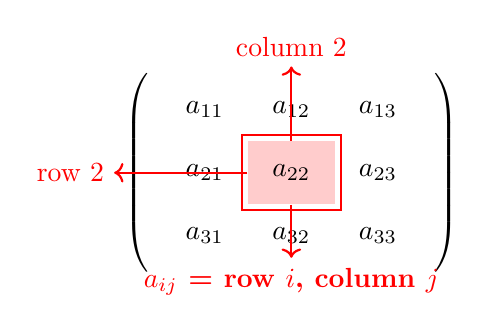
\begin{tikzpicture}[scale=0.9]
\matrix (m) [matrix of math nodes, left delimiter=(, right delimiter=), nodes={minimum width=1.1cm, minimum height=0.8cm}] {
  a_{11} & a_{12} & a_{13} \\
  a_{21} & |[fill=red!20]| a_{22} & a_{23} \\
  a_{31} & a_{32} & a_{33} \\
};
\node[draw=red, thick, fit=(m-2-2), inner sep=2pt] {};
\draw[->,red,thick] (m-2-2) -- ++(0,-1.2) node[below] {\textbf{$a_{ij}$ = row $i$, column $j$}};
\draw[->,red,thick] (m-2-2) -- ++(-2.5,0) node[left] {row 2};
\draw[->,red,thick] (m-2-2) -- ++(0,1.5) node[above] {column 2};
\end{tikzpicture}
\end{center}

\vfill
For $a_{22}$: first index = row number (2), second index = column number (2).
\end{frame}

\begin{frame}[fragile]{Visual Proof: $\operatorname{tr}(AB) = \operatorname{tr}(BA)$ — Setup}
Consider $A$ is $2 \times 3$ and $B$ is $3 \times 2$:

\vfill
\begin{center}
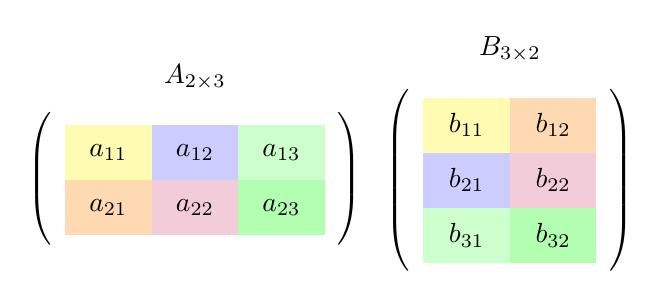
\begin{tikzpicture}[scale=0.8]
% Matrix A
\matrix (A) at (0,0) [matrix of math nodes, left delimiter=(, right delimiter=), nodes={minimum width=1.1cm, minimum height=0.7cm}] {
  |[fill=yellow!30]| a_{11} & |[fill=blue!20]| a_{12} & |[fill=green!20]| a_{13} \\
  |[fill=orange!30]| a_{21} & |[fill=purple!20]| a_{22} & |[fill=green!30]| a_{23} \\
};
\node[above=0.2cm of A] {$A_{2\times 3}$};

% Matrix B
\matrix (B) at (5,0) [matrix of math nodes, left delimiter=(, right delimiter=), nodes={minimum width=1.1cm, minimum height=0.7cm}] {
  |[fill=yellow!30]| b_{11} & |[fill=orange!30]| b_{12} \\
  |[fill=blue!20]| b_{21} & |[fill=purple!20]| b_{22} \\
  |[fill=green!20]| b_{31} & |[fill=green!30]| b_{32} \\
};
\node[above=0.2cm of B] {$B_{3\times 2}$};
\end{tikzpicture}
\end{center}

\vfill
First, compute $AB$ (will be $2 \times 2$):

Diagonal entries:
\begin{align*}
(AB)_{11} &= \textcolor{orange}{a_{11}b_{11}} + \textcolor{blue}{a_{12}b_{21}} + \textcolor{green!50!black}{a_{13}b_{31}} \\
(AB)_{22} &= \textcolor{orange}{a_{21}b_{12}} + \textcolor{purple!80!black}{a_{22}b_{22}} + \textcolor{green!50!black}{a_{23}b_{32}}
\end{align*}
\end{frame}

\begin{frame}{Visual Proof: $\operatorname{tr}(AB)$}
$$\operatorname{tr}(AB) = (AB)_{11} + (AB)_{22}$$

\vfill
\begin{align*}
&= (a_{11}b_{11} + a_{12}b_{21} + a_{13}b_{31}) \\
&\quad + (a_{21}b_{12} + a_{22}b_{22} + a_{23}b_{32})
\end{align*}

\vfill
This is the sum of all \x{color-matched pairs}.
\end{frame}

\begin{frame}[fragile]{Visual Proof: Now Compute $BA$}
$BA$ is $3 \times 3$:

\begin{center}
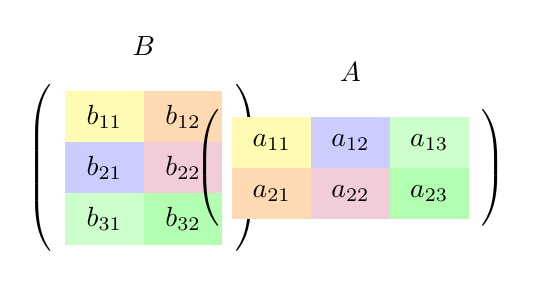
\begin{tikzpicture}[scale=0.75]
% Matrix B
\matrix (B) at (0,0) [matrix of math nodes, left delimiter=(, right delimiter=), nodes={minimum width=1cm, minimum height=0.65cm}] {
  |[fill=yellow!30]| b_{11} & |[fill=orange!30]| b_{12} \\
  |[fill=blue!20]| b_{21} & |[fill=purple!20]| b_{22} \\
  |[fill=green!20]| b_{31} & |[fill=green!30]| b_{32} \\
};
\node[above=0.2cm of B] {$B$};

% Matrix A
\matrix (A) at (3.5,0) [matrix of math nodes, left delimiter=(, right delimiter=), nodes={minimum width=1cm, minimum height=0.65cm}] {
  |[fill=yellow!30]| a_{11} & |[fill=blue!20]| a_{12} & |[fill=green!20]| a_{13} \\
  |[fill=orange!30]| a_{21} & |[fill=purple!20]| a_{22} & |[fill=green!30]| a_{23} \\
};
\node[above=0.2cm of A] {$A$};
\end{tikzpicture}
\end{center}

\vfill
Diagonal entries of $BA$:
\begin{align*}
(BA)_{11} &= b_{11}a_{11} + b_{12}a_{21} \\
(BA)_{22} &= b_{21}a_{12} + b_{22}a_{22} \\
(BA)_{33} &= b_{31}a_{13} + b_{32}a_{23}
\end{align*}
\end{frame}

\begin{frame}{Visual Proof: $\operatorname{tr}(BA)$}
$$\operatorname{tr}(BA) = (BA)_{11} + (BA)_{22} + (BA)_{33}$$

\vfill
\begin{align*}
&= (b_{11}a_{11} + b_{12}a_{21}) \\
&\quad + (b_{21}a_{12} + b_{22}a_{22}) \\
&\quad + (b_{31}a_{13} + b_{32}a_{23})
\end{align*}

\vfill
By commutativity of multiplication ($a_{ij}b_{kl} = b_{kl}a_{ij}$):

\begin{align*}
&= (a_{11}b_{11} + a_{21}b_{12}) + (a_{12}b_{21} + a_{22}b_{22}) + (a_{13}b_{31} + a_{23}b_{32})
\end{align*}

\vfill
This is \x{exactly the same} sum as $\operatorname{tr}(AB)$!

$$\boxed{\operatorname{tr}(AB) = \operatorname{tr}(BA)}$$
\end{frame}

\begin{frame}{Using Trace to Prove Dimension Well-Defined}
\begin{thm}
If $W$ has two bases with $m$ and $n$ vectors, then $m = n$.
\end{thm}

\vfill
\textbf{Proof strategy}:
\begin{enumerate}
\item Write one basis in terms of the other (change-of-basis matrices)
\item Use left cancellation: these matrices compose to identity
\item Use trace to count sizes
\end{enumerate}
\end{frame}

\begin{frame}{Proof: Change-of-Basis Matrices}
Let:
\begin{itemize}
\item Basis 1: $U = \begin{pmatrix} | & & | \\ \mathbf{u}_1 & \cdots & \mathbf{u}_m \\ | & & | \end{pmatrix}$
\item Basis 2: $V = \begin{pmatrix} | & & | \\ \mathbf{v}_1 & \cdots & \mathbf{v}_n \\ | & & | \end{pmatrix}$
\end{itemize}

\vfill
Since Basis 2 \x{spans} $W$, each $\mathbf{u}_j$ can be written using $\mathbf{v}_i$'s:

$$U = V P$$

for some $n \times m$ matrix $P = \begin{pmatrix} | & & | \\ \mathbf{p}_1 & \cdots & \mathbf{p}_m \\ | & & | \end{pmatrix}$.

\vfill
Column $\mathbf{p}_j$ provides \x{coefficients} to write $\mathbf{u}_j$ as combination of $\mathbf{v}_i$'s!
\end{frame}

\begin{frame}{Proof: The Reverse Direction}
Similarly, since Basis 1 \x{spans} $W$:

$$V = U Q$$

for some $m \times n$ matrix $Q = \begin{pmatrix} | & & | \\ \mathbf{q}_1 & \cdots & \mathbf{q}_n \\ | & & | \end{pmatrix}$.

\vfill
Column $\mathbf{q}_i$ provides \x{coefficients} to write $\mathbf{v}_i$ as combination of $\mathbf{u}_j$'s!
\end{frame}

\begin{frame}{Proof: Composing the Changes}
Substitute $V = UQ$ into $U = VP$:

$$U = VP = (UQ)P = U(QP)$$

\vfill
Since $U$ has \x{linearly independent} columns, by \x{left cancellation}:

$$QP = I_m$$

(an $m \times m$ identity matrix)

\vfill
Similarly, substitute $U = VP$ into $V = UQ$:

$$V = UQ = (VP)Q = V(PQ)$$

By left cancellation:

$$PQ = I_n$$

(an $n \times n$ identity matrix)
\end{frame}

\begin{frame}{Proof: Using Trace}
We have:
\begin{itemize}
\item $QP = I_m$ (size $m \times m$)
\item $PQ = I_n$ (size $n \times n$)
\end{itemize}

\vfill
Taking traces:
$$\operatorname{tr}(QP) = \operatorname{tr}(I_m) = m$$
$$\operatorname{tr}(PQ) = \operatorname{tr}(I_n) = n$$

\vfill
But by the trace property:
$$\operatorname{tr}(QP) = \operatorname{tr}(PQ)$$

\vfill
Therefore: $m = n$ $\square$

\vfill
\x{Any two bases have the same size!}
\end{frame}

\begin{frame}{Dimension is Now Well-Defined}
\begin{defi}[Dimension]
The \x{dimension} of a subspace $W$ is the number of vectors in any basis:

$$\dim(W) = \text{number of vectors in any basis for } W$$

This is \x{independent of which basis} we choose!
\end{defi}

\vfill
\x{Examples}:
\begin{itemize}
\item $\dim(\mathbb{R}^n) = n$ (standard basis has $n$ vectors)
\item $\dim(\operatorname{Col}(A))$ = number of vectors in any basis for column space
\item $\dim(\{\mathbf{0}\}) = 0$ (zero subspace)
\end{itemize}
\end{frame}

% ═══════════════════════════════════════
% §10 RANK IS WELL-DEFINED
% ═══════════════════════════════════════
\section{Rank is Well-Defined}

\begin{frame}{Connecting Rank to Dimension}
\begin{thm}[Rank = Dimension]
For any matrix $A$:
$$\operatorname{rank}(A) = \dim(\operatorname{Col}(A))$$
\end{thm}

\vfill
\textbf{Proof}:

From §8, cross-filling produces $A = UV$ where:
\begin{itemize}
\item $U$ has $r$ columns
\item Columns of $U$ form a \x{basis} for $\operatorname{Col}(A)$
\item Therefore $\dim(\operatorname{Col}(A)) = r$
\end{itemize}

\vfill
By Lecture 3 definition:
$$\operatorname{rank}(A) = r \text{ (number of rank-one pieces)}$$

\vfill
Therefore: $\operatorname{rank}(A) = \dim(\operatorname{Col}(A))$ $\square$
\end{frame}

\begin{frame}{Rank is Well-Defined!}
\x{Why?} Because:
\begin{enumerate}
\item $\operatorname{rank}(A) = \dim(\operatorname{Col}(A))$ (just proved)
\item $\dim(\operatorname{Col}(A))$ is well-defined (all bases have same size)
\item Therefore $\operatorname{rank}(A)$ is well-defined!
\end{enumerate}

\vfill
\x{Different cross-filling runs} (different pivot choices) may give:
\begin{itemize}
\item Different $U$ matrices
\item Different $V$ matrices
\item Different rank-one pieces $R_1, R_2, \ldots$
\end{itemize}

\vfill
\x{But they all give}:
\begin{itemize}
\item \x{Same number $r$ of pieces} (since $r = \dim(\operatorname{Col}(A))$)
\item \x{Same column space} $\operatorname{Col}(A)$
\end{itemize}
\end{frame}

\begin{frame}{Example: Independence of Pivot Choices}
$$A = \begin{pmatrix} 2 & 4 \\ 1 & 2 \end{pmatrix}$$

\vfill
\x{Pivot choice 1} (position $(1,1)$):
$$A = \begin{pmatrix} 2 \\ 1 \end{pmatrix}\begin{pmatrix} 1 & 2 \end{pmatrix}$$
One piece $\to$ rank = 1

\vfill
\x{Pivot choice 2} (position $(2,2)$):
$$A = \begin{pmatrix} 1 \\ 0.5 \end{pmatrix}\begin{pmatrix} 2 & 4 \end{pmatrix}$$
One piece $\to$ rank = 1

\vfill
\x{Both give rank 1} because:
$$\operatorname{Col}(A) = \left\{ t\begin{pmatrix} 2 \\ 1 \end{pmatrix} : t \in \mathbb{R} \right\}$$

is a \x{1-dimensional} line!
\end{frame}

% ═══════════════════════════════════════
% §11 SUMMARY
% ═══════════════════════════════════════
\section{Summary}

\begin{frame}{What We Achieved Today}
\x{From Algorithm to Geometry}:

\vfill
\textbf{Lecture 3}: Rank was \x{algorithmic} (count pieces from cross-filling)
\begin{itemize}
\item Problem: Different pivot choices might give different counts
\end{itemize}

\vfill
\textbf{Lecture 4}: Rank is \x{geometric}:
$$\boxed{\operatorname{rank}(A) = \dim(\operatorname{Col}(A))}$$

\begin{itemize}
\item Solution: Dimension is well-defined (all bases same size)
\item Therefore rank is well-defined!
\end{itemize}

\vfill
\x{Key insight}: Cross-filling \x{finds a basis} for $\operatorname{Col}(A)$!
\end{frame}

\begin{frame}{The Conceptual Framework}
\begin{center}
\begin{tabular}{|l|p{3.5cm}|p{3.5cm}|}
\hline
& \textbf{Descriptive} & \textbf{Constructive} \\
\hline
\textbf{Definition} & List constraints & Give recipe \\
\hline
\textbf{Example} & Null space: $\{x : Ax=0\}$ & Column space: $\{Ax : x \in \mathbb{R}^n\}$ \\
\hline
\textbf{Strength} & Verify membership & Generate members \\
\hline
\end{tabular}
\end{center}

\vfill
\x{Basis} = minimal spanning set = maximal independent set

\vfill
\x{Dimension} = size of any basis (well-defined!)

\vfill
\x{Rank} = dimension of column space = number of basis vectors from cross-filling
\end{frame}

\begin{frame}{Tools We Developed}
\begin{enumerate}
\item \x{Two Languages} for sets: Descriptive $\leftrightarrow$ Constructive
\item \x{Subspaces}: Flat spaces through origin, closed under linear combinations
\item \x{Linear Independence}: No redundancy, minimum generators
\item \x{Basis}: Linearly independent + spans = unique coordinates
\item \x{Left Cancellation}: $UP = UQ \Rightarrow P = Q$ (for independent $U$)
\item \x{Cross-filling produces basis}: Pivot structure $\to$ independence
\item \x{Trace property}: $\operatorname{tr}(AB) = \operatorname{tr}(BA)$ (visual proof)
\item \x{Dimension well-defined}: All bases same size (using trace)
\item \x{Rank = Dimension}: Geometric meaning of rank
\end{enumerate}
\end{frame}

\end{document}
